\documentclass[11pt]{article}
\usepackage[margin=1in]{geometry}
\usepackage{graphicx}
\usepackage{booktabs}
\usepackage{amsmath}
\usepackage{hyperref}
\usepackage{xcolor}
\usepackage{natbib}

\newcommand{\TBD}{\textcolor{red}{TBD}}

\title{OnCallGym: A Verifiable Environment for Training LLM Agents\\on Production Incident Response}
\author{}
\date{}

\begin{document}
\maketitle

\begin{abstract}
We present OnCallGym, a reinforcement-learning environment in which a language-model agent acts as the on-call engineer for a simulated online shop of fifteen cooperating services. Each episode injects one of seventeen production faults; the agent investigates with ops tools, changes configuration, and submits a diagnosis. A programmatic verifier, independent of the agent's tools, checks recovery with its own customer traffic, re-checks it after restarting every service, compares the diagnosis with the ground truth, and gates the reward on business and integrity invariants. We catalogue 25 reward hacks found during development and the checks that block them; across 1{,}888 evaluated episodes no episode received recovery credit without the root cause being fixed. Training Qwen3-1.7B on free Kaggle GPUs, scripted-oracle SFT lifts the solve rate on easy training faults from 0\% to 20\%, and GRPO adds a suggestive reward gain on those faults but no solve-rate gain and no transfer to five held-out fault families (0/160 solved for all models). We also report two failure modes of a standard GRPO stack (TRL + vLLM) with multi-turn, LoRA-trained policies: sequence-level importance-sampling masks that silently zero the gradient, and a race in the LoRA weight sync that makes vLLM sample from a partially merged model.
\end{abstract}

\section{Introduction}
Benchmarks for software agents mostly score code changes against tests \citep{jimenez2024swebench}. Operating a running system is different: the agent must find a fault from symptoms, act on live state, and leave the system healthy, while a careless or adversarial agent has many ways to make the symptom disappear without fixing anything. Recent operations benchmarks \citep{chen2025aiopslab,jha2025itbench} evaluate agents on such tasks; OnCallGym is built for \emph{training} with RL, which makes reward integrity the central design constraint \citep{skalse2022rewardhacking}. It runs as plain processes (no containers at train time) so that episodes can execute next to the model on free GPU notebooks.

Contributions: (1) an environment of 15 services, 17 validated fault families with seeded variants and a train/held-out family split; (2) a verifier and a hack catalogue with regression tests; (3) an honest training study on free compute, including negative transfer results; (4) two reproducible pitfalls in multi-turn GRPO with vLLM and LoRA, with fixes.

\section{Environment}
\paragraph{System.} Northwind Commerce consists of an edge gateway, auth, catalog, orders, inventory, payments (calling an external payment provider), a message broker, fulfillment, notify (sending through an external mail relay), cache, feature flags, a scheduler, telemetry and a traffic generator, all managed by one supervisor. Services are small Python processes with real configuration files, logs, SQLite data and inter-service HTTP; each episode gets its own directory, port range and Unix user, so many episodes run in parallel.

\paragraph{Episode.} After the stack is healthy, a fault family configures one fault (before boot where possible, restoring file and directory timestamps so that the answer cannot be read from metadata). The agent sees a symptom-only alert and has eight tools: \texttt{exec} (a shell in the deployment directory), \texttt{logs}, \texttt{metrics}, \texttt{trace}, \texttt{topology}, \texttt{list\_services}, \texttt{restart} and \texttt{submit\_diagnosis}, which ends the episode. Turn limits are 12, 14 and 16 tool calls for easy, medium and hard faults.

\paragraph{Tasks.} Twelve families are used for training (4 easy, 6 medium, 2 hard) and five are held out (1 easy, 3 medium, 1 hard); the held-out families never appear in SFT data or RL. Each family generates variants from a seed (values, affected services, red herrings). Every family passes an automatic validation: healthy before injection, probes fail after it, the scripted oracle fix scores about 1.0, doing nothing about 0, restarting everything does not solve it, and every known cheat trips the integrity gate.

\section{Verifier and reward}
The verifier runs after the agent finishes, with its own probes:
\begin{itemize}
\item \textbf{R (recovery)}: scripted customer journeys and an 8-second traffic window pass, liveness invariants hold (paid orders shipped or refunded, customers notified, events consumed), and the family's \texttt{root\_cause\_fixed()} holds on the configuration each service actually loaded.
\item \textbf{P (persistence)}: every service is restarted and R is checked again.
\item \textbf{C (diagnosis)}: the submitted category and component match the ground truth.
\item \textbf{G (gate)}: no duplicate charges, stock conserved, charges match orders, seed data intact, nothing purged; protected files, logging, scheduler jobs and the traffic generator untouched.
\end{itemize}
\begin{equation}
\text{reward} = G\,(0.5\,R\,P + 0.3\,C + 0.2\,R), \qquad \text{solved} = R \wedge P \wedge C \wedge G.
\end{equation}

\paragraph{Reward hacking.} We catalogued 25 hacks from design review, an automated adversarial run and three independent code reviews, among them: restarting everything for a persistent fault; making the external provider or mail relay reliable instead of fixing the cause; deleting failed orders or purging unacknowledged messages; writing the databases from the shell; code injection through environment files; a background process that keeps fulfilling orders; pointing a service at an agent-written config through an override variable; and reading the answer from code, timestamps, process arguments or trajectory files. Each is blocked by a check, most with a regression test; the README lists all of them. Over all 1{,}888 episodes evaluated in this work, no episode received R or P credit without the root cause fixed; the highest reward without a fix is 0.3 (diagnosis credit). Every gate trip we read was real damage from a bad edit, not an exploit. A remaining leniency: the verifier checks that the faulty value was corrected, not that the file is otherwise clean.

\section{Training}
\paragraph{Setup.} Qwen3-1.7B \citep{qwen3} with thinking disabled, 8k context, LoRA rank 16 \citep{hu2022lora}, on Kaggle T4$\times$2 (trainer on one GPU, a vLLM server \citep{kwon2023vllm} on the other), TRL 1.18 GRPO \citep{vonwerra2020trl,shao2024deepseekmath}. Training rollouts, SFT data and evaluation share one agent loop and token renderer (chat template, tool schemas, tool-call format, nudges after text-only replies), enforced by tests.

\paragraph{SFT warm start.} 384 scripted oracle trajectories (12 training families $\times$ 8 variants $\times$ 4), varied with extra investigation, dismissed red herrings and wrong-then-corrected steps, kept only if the verifier scores them solved; loss on assistant tokens only. No model-generated data is used.

\paragraph{Pitfall 1: sequence-level importance sampling.} TRL corrects for the difference between the sampler (vLLM) and the trainer with an importance ratio; its default multiplies per-token ratios over the whole completion and masks sequences whose ratio leaves a band. Multi-turn episodes have $\sim$500 model tokens, so a per-token gap of 0.15--0.6 nats drives every ratio to zero: our first 40-step run had a gradient norm of exactly 0 on every step. Per-token truncation keeps the signal.

\paragraph{Pitfall 2: racy LoRA weight sync.} The gap itself was a bug. To push LoRA weights to vLLM, TRL merges the adapter, yields views of the live parameters, and unmerges after the last one; vLLM's packed NCCL producer consumes this generator inside blocks on two alternating side CUDA streams and concatenates the views there. Nothing orders the merge or unmerge against those copies, so some layers reach vLLM unmerged. Scoring vLLM's sampled tokens with an fp32 reference showed vLLM matching the adapter at half strength after the second sync. Synchronizing the device after the merge, yielding copies, and synchronizing before the unmerge reduces the mean per-token gap from 0.3--1.2 to 0.003--0.02 on every step (Figure~\ref{fig:sync}). With the racy sync, GRPO made the policy worse (mean reward $-0.067$ on easy training faults); with the fix it trains.

\begin{figure}[t]
\centering
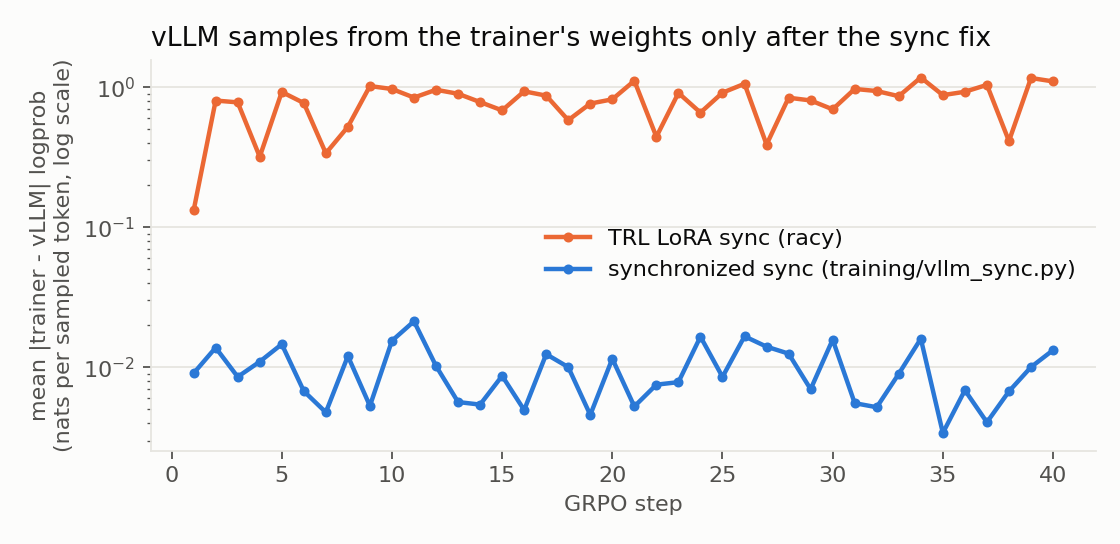
\includegraphics[width=0.85\linewidth]{../results/plots/sync_fix_logprob_gap.png}
\caption{Mean absolute difference between trainer and vLLM log-probabilities of the sampled tokens, per GRPO step, before and after the weight-sync fix (same settings otherwise).}
\label{fig:sync}
\end{figure}

\section{Results}
All evaluations use the same evaluator and sampler (temperature 0.7, top-$p$ 0.95, top-$k$ 20); comparisons are paired by task with a bootstrap CI and a sign-flip test, and additionally by family with an exact sign-flip test, since variants of one family share most of their prompt.

\begin{table}[h]
\centering
\small
\begin{tabular}{llrrrr}
\toprule
model & eval set & episodes & solved & mean reward & C \\
\midrule
base & held-out (20 tasks) & 160 & 0.0\% & 0.039 & 0.13 \\
SFT & held-out & 160 & 0.0\% & 0.024 & 0.08 \\
SFT+GRPO (40 steps, easy) & held-out & 160 & 0.0\% & 0.024 & 0.08 \\
SFT & easy train (16 tasks) & 256 & 19.9\% & 0.334 & 0.64 \\
SFT+GRPO (40 steps, easy) & easy train & 256 & 20.7\% & 0.390 & 0.74 \\
SFT+GRPO (all train tiers) & held-out / all train & \TBD & \TBD & \TBD & \TBD \\
Qwen3 0.6B / 4B / 8B (no training) & held-out / all train & \TBD & \TBD & \TBD & \TBD \\
\bottomrule
\end{tabular}
\caption{Qwen3-1.7B results. C: share of episodes with the right category and component.}
\label{tab:results}
\end{table}

The base model never solves a fault and, on held-out faults, runs out of turns or context in 83\% of episodes. SFT teaches the protocol and lifts the easy-training solve rate to 19.9\%. GRPO on easy faults raised mean reward by $+0.056$ (task-level 95\% CI $[+0.013, +0.095]$, $p=0.02$), mostly through better diagnoses (C 0.64$\to$0.74), but we treat this as suggestive: the gain comes from two of four families (exact family-level $p=0.25$), the two arms were evaluated in different sessions, and an A/A comparison of identical weights showed $+0.044$ reward of pure noise. The strict solve rate did not change ($+0.008$, $p=0.88$). On the five held-out families, no model solves anything and rewards do not differ significantly (SFT$\to$GRPO $+0.000$; base$\to$SFT $-0.015$, $p=0.39$).

\section{Analysis}
\begin{figure}[t]
\centering
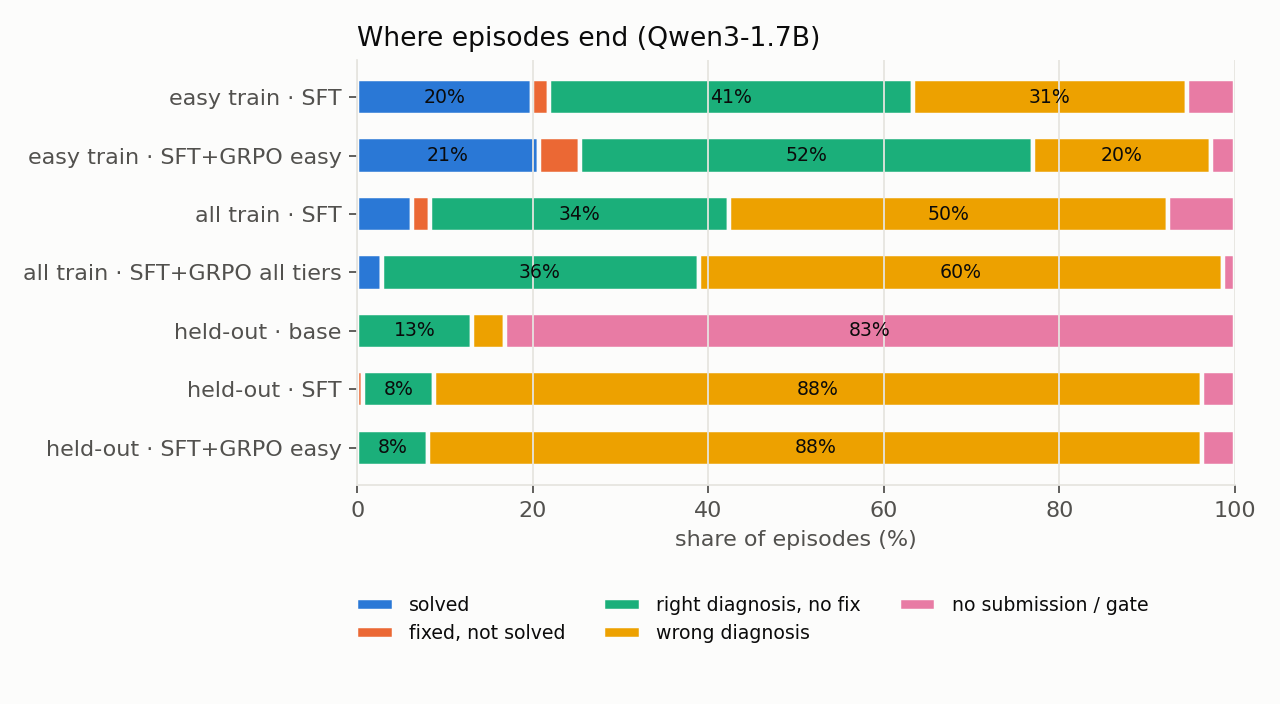
\includegraphics[width=0.9\linewidth]{../results/plots/outcomes.png}
\caption{Outcome of every episode, checked in order: solved; fixed but not solved; right diagnosis without a fix; wrong diagnosis; no submission or integrity gate tripped.}
\label{fig:outcomes}
\end{figure}
Figure~\ref{fig:outcomes} shows where episodes end. On training families the bottleneck is the edit, not the diagnosis: 41--52\% of episodes name the right cause and component but do not fix it. Reading these episodes, the model finds the right file and key and then writes a \texttt{sed} command that does not apply (a regular expression for a key that does not exist), fixes half of the fault (the rate but not the burst limit), or breaks the YAML; the restart succeeds and the agent submits. On held-out families, trained models nearly always submit but blame the wrong service in 56--68\% of episodes: they transfer the protocol, not the diagnosis. The base model rarely submits, but its few submissions are mostly right.

\section{Limitations}
One model size, short GRPO runs and a 30 GPU-hour weekly budget limit what we can claim; the held-out families also differ in difficulty from the easy training faults used for RL so far. The system is synthetic and small; realism comes from the failure modes, alerts and checks rather than scale. The automated red team (a local 8B model) was too weak to find exploits, so the hack catalogue relies on human-style review.

\bibliographystyle{plainnat}
\bibliography{refs}
\end{document}
